\section{L3 Cache Size Sensitivity}
\label{sec:results:l3size_sensitivity}

In this section, we cover an experiment where we run all 4-core workloads with varying L3 cache size.
While we have already shown in section~\ref{sec:methodology:processor_model} that our simulated model is realistic compared to current processor architectures, we want to explore how algorithm performance changes when we constrain available L3 cache.
This experiment uses the same simulated system as in the cache partitioning experiment, section~\ref{sec:results:cache_partition}.
We use four different L3 sizes; 4MB, 2MB, 1MB, and 0.5MB.
Table~\ref{tbl:processor_model:l3} shows detailed information about the two larger configurations.
The details for the two smaller configurations are equal to the L2 configurations of the same size, shown in table~\ref{tbl:processor_model:l2}, but with an associativity of 32.
When we reduce the size of the shared cache level, we keep the associativity constant.
This results in fewer sets in the cache and hence, more addresses map to the same set.
Fewer sets cause increased pressure on each set.
We expect to see some of the algorithms further their improvement over LRU in this situation.
And we expect PIPP, which already has shown bad performance compared to LRU, to continue this trend.

Figure~\ref{fig:results:l3} present the speedup of all algorithms normalized to LRU for varying shared cache size.
DRRIP is the algorithm that shows least variation across the various shared cache sizes.
Figure~\ref{fig:results:l3:drrip} shows DRRIP performing comparable to LRU in all cases, with a negligible increase of 0.3\% in the 1MB case.
TADIP that in the baseline scenario performs as good as LRU, seems to suffer from the increased set pressure, with increasingly worse performance as the cache size decreases.
In our implementation, we scale the number of duel-sets relative to the total number of cache sets.
Hence, for both DRRIP and TADIP the fraction of duel sets is constant across the various L3 configurations.

As expected the performance of PIPP decreases as the set pressure increases, shown in figure~\ref{fig:results:l3:pipp}.
We have previously, in section~\ref{sec:results:cache_partition}, postulated that the potentially short lifetime of blocks in a PIPP managed cache may be the cause of the performance decrease caused by PIPP compared to LRU.
This experiment further shows that when the number of accesses to a single set increases the performance of PIPP further decreases compared to LRU.
The MPKI in the 0.5MB cases, not shown here, is over 50\% worse than the LRU case, compared to only 20\% worse in the 4MB case.
PIPP-min8, a modified version of PIPP, have previously been shown to improve performance over normal PIPP replacement.
This is also the case when reducing shared cache size.
Figure~\ref{fig:results:l3:pipp-min8} shows that PIPP-min8 not only performs as good as LRU in the base experiment, but with increased set pressure actually performs better than LRU.
With a 0.5MB L3 cache, the modified PIPP algorithm performs 4\% better than LRU measured in STP.
In the same configuration, the unmodified algorithm performs about 18\% worse compared to LRU.
This result clearly shows the advantage of the extended block lifetime in the modified PIPP algorithm, and at the same time points an fundamental performance problem with PIPP.

\begin{figure}[!htb]
    \centering
    \begin{subfigure}[b]{0.5\textwidth}
        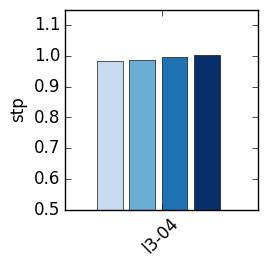
\includegraphics[width=\textwidth]{figures/results/speedup/l3-stp-04M-tadip-l3}
        \caption{Speedup of TADIP normalized to LRU.}
        \label{fig:results:l3:tadip}
    \end{subfigure}%
    \begin{subfigure}[b]{0.5\textwidth}
        \includegraphics[width=\textwidth]{figures/results/speedup/l3-stp-04M-drrip-3-l3}
        \caption{Speedup of DRRIP normalized to LRU.}
        \label{fig:results:l3:drrip}
    \end{subfigure}
\end{figure}
\clearpage
\begin{figure}[!htb]
    \ContinuedFloat
    \begin{subfigure}[b]{0.5\textwidth}
        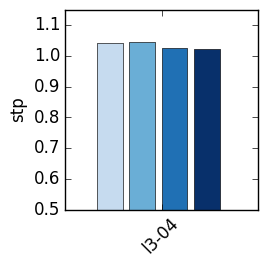
\includegraphics[width=\textwidth]{figures/results/speedup/l3-stp-04M-ucp-l3}
        \caption{Speedup of UCP normalized to LRU.}
        \label{fig:results:l3:ucp}
    \end{subfigure}%
    \begin{subfigure}[b]{0.5\textwidth}
        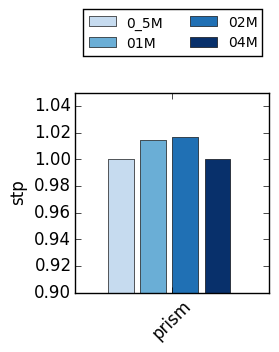
\includegraphics[width=\textwidth]{figures/results/speedup/l3-stp-04M-prism-l3}
        \caption{Speedup of PriSM normalized to LRU.}
        \label{fig:results:l3:prism}
    \end{subfigure}
    \begin{subfigure}[b]{0.5\textwidth}
        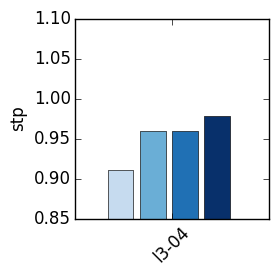
\includegraphics[width=\textwidth]{figures/results/speedup/l3-stp-04M-pipp-l3}
        \caption{Speedup of PIPP normalized to LRU.}
        \label{fig:results:l3:pipp}
    \end{subfigure}%
    \begin{subfigure}[b]{0.5\textwidth}
        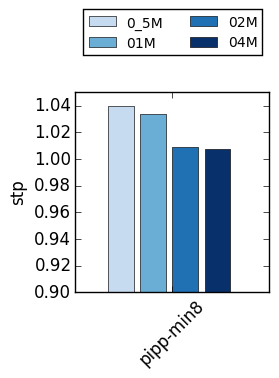
\includegraphics[width=\textwidth]{figures/results/speedup/l3-stp-04M-pipp-min8-l3}
        \caption{Speedup of PIPP-min8 normalized to LRU.}
        \label{fig:results:l3:pipp-min8}
    \end{subfigure}
    \caption{Speedup of cache partition algorithms normalized to LRU with decreasing shared L3 size}
    \label{fig:results:l3}
\end{figure}

\begin{figure}[!htb]
    \centering
    \begin{subfigure}[b]{0.5\textwidth}
        \includegraphics[width=\textwidth]{figures/results/speedup/l3-mkpi-04M-prism-l3}
        \caption{MPKI under PriSM normalized to LRU.}
        \label{fig:results:l3:mpki-prism}
    \end{subfigure}%
    \begin{subfigure}[b]{0.5\textwidth}
        \includegraphics[width=\textwidth]{figures/results/speedup/l3-mkpi-04M-ucp-l3}
        \caption{MPKI under UCP normalized to LRU.}
        \label{fig:results:l3:mpki-ucp}
    \end{subfigure}
\end{figure}

Next, we have PriSM, which shows a slight performance increase with the 2MB and 1MB cache, shown in figure~\ref{fig:results:l3:prism}. 
At both 4MB and 0.5MB PriSM performs as good as LRU.
Figure~\ref{fig:results:l3:mpki-prism} shows the MPKI for PriSM.
From this figure, we observe that PriSM in all configurations causes the same number of misses as LRU.
This is true even when PriSM shows an performance increase measured in STP.
Finally, the performance of UCP shown in figure~\ref{fig:results:l3:ucp}. 
In previous sections (\ref{sec:results:cache_partition} and \ref{sec:results:l2size_sensitivity}) we have shown that UCP is the top performer of our algorithms when measured in STP.
This is also the case when the size of shared cache is lowered.
We observe that UCP increases performance compared to LRU in both the 2MB and 1MB case, in the 0.5MB case is comparable to the 1MB case.
Interestingly, figure~\ref{fig:results:l3:mpki-ucp} shows that while UCP increases performance compared to LRU it also causes more misses, shown by an increase in MPKI.
Previous experiments have also shown this effect, and we have detailed a possible cause for this effect in section~\ref{sec:results:cache_partition}.
